\subsection{Результат внедрения}
В рамках данной работы структура данных Сито-индекс была внедрена в платформу для доступа к данным Apache Hudi \fbox{ссылка на гитхаб}.

В данном разделе представлены результаты сравнения скорости работы точечных и интервальных запросов с использованием упрощенных сводок и Сито-индекса для таблиц разного размера. Тестовый набор данных был сгенерирован с использованием бенчмарка TPC-H \fbox{ссылка}, запросы производились к таблице {<<lineitem>>} по атрибуту {<<shipdate>>}.

В процессе тестирования индекс был построен для двух таблиц разного размера: первые 20 миллионов строк (первый набор данных) и первые 600 миллионов строк (второй набор данных) из таблицы {<<lineitem>>}. Тестовый вычислительный кластер Spark состоял из одного узла, который был ограничен объемом оперативной памяти в 2 ГБ. Это позволило проверить возможность индексации таблицы из 20 миллионов записей с полной загрузкой всех значений атрибута в память и возможность построения индекса для таблицы из 600 миллионов записей, размер индексируемого атрибута такой таблицы не умещается в 2 ГБ оперативной памяти.

Размер индекса для первого набора данных составил 1,5 МБ при общем размере индексируемого атрибута в 80 МБ (20 миллионов значений по 4 Б), а для второго — 52 МБ при общем размере индексируемого атрибута 2,2 ГБ (600 миллионов значений по 4 Б). При этом размер индекса составил примерно $6\%$ от исходного размера индексируемого атрибута.

\begin{figure}[h]
    \centering
    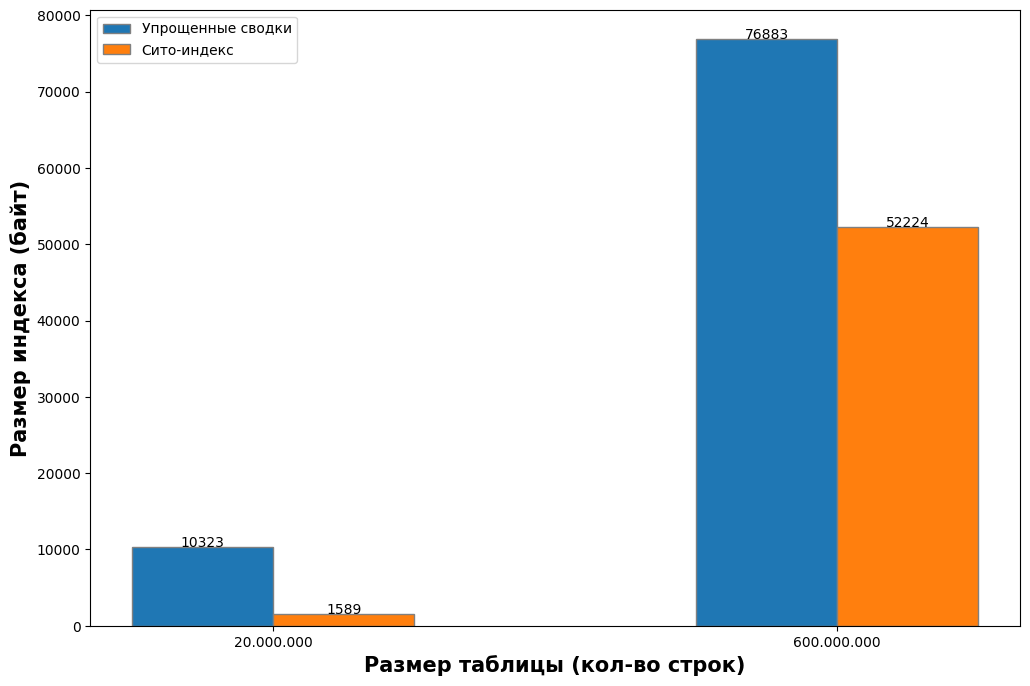
\includegraphics[scale=0.62]{4_index_size.png}
    \caption{\centering{Сравнение итогового размера упрощенных сводок и Сито-индекса на файловой системе для двух таблицах разного размера}}
\end{figure}

Причина, по которой итоговый размер упрощенных сводок получился больше размера Сито-индекса заключается в реализации упрощенных сводок в Apache Hudi \fbox{ссылка}, каждая запись содержит полное название файловой группы (\fbox{ссылка}), в то время как авторская реализация Сито-индекса кодирует каждый идентификатор файловой группы используя ассоциативный массив, что позволяет сократить использование памяти. 

Далее представлено сравнение скорости выполнения запроса для точечных и интервальных запросов.

\begin{figure}[p]
    \centering
    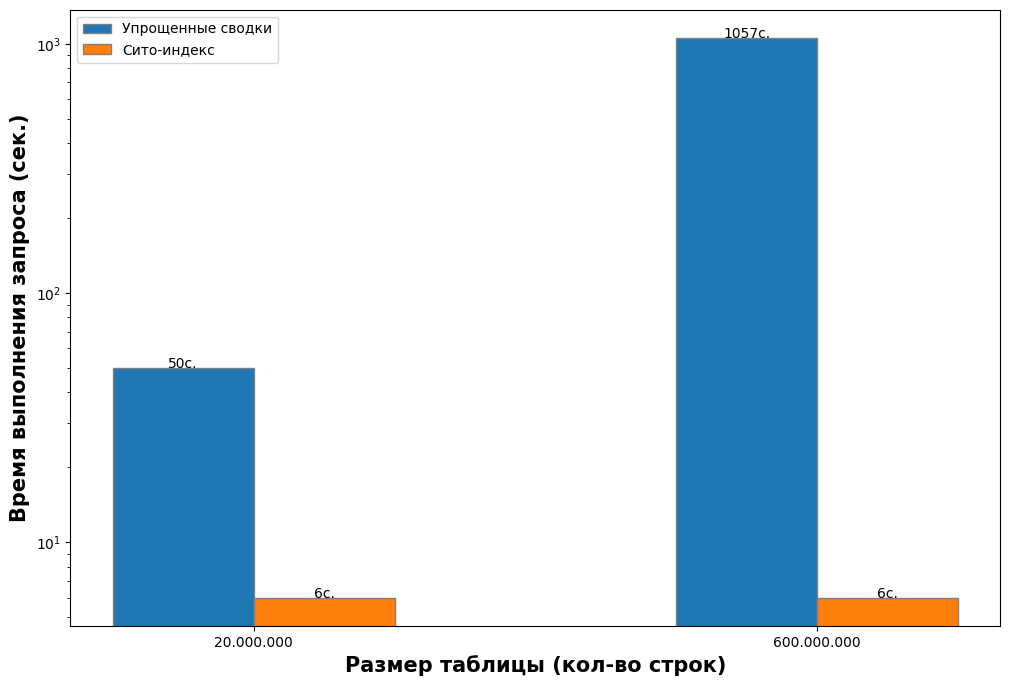
\includegraphics[scale=0.62]{1_point_query.png}
    \caption{\centering{Сравнение времени выполнения точечного запроса с использованием упрощенных сводок и Сито-индекса на двух таблицах разного размера}}
\end{figure}


\begin{figure}[p]
    \centering
    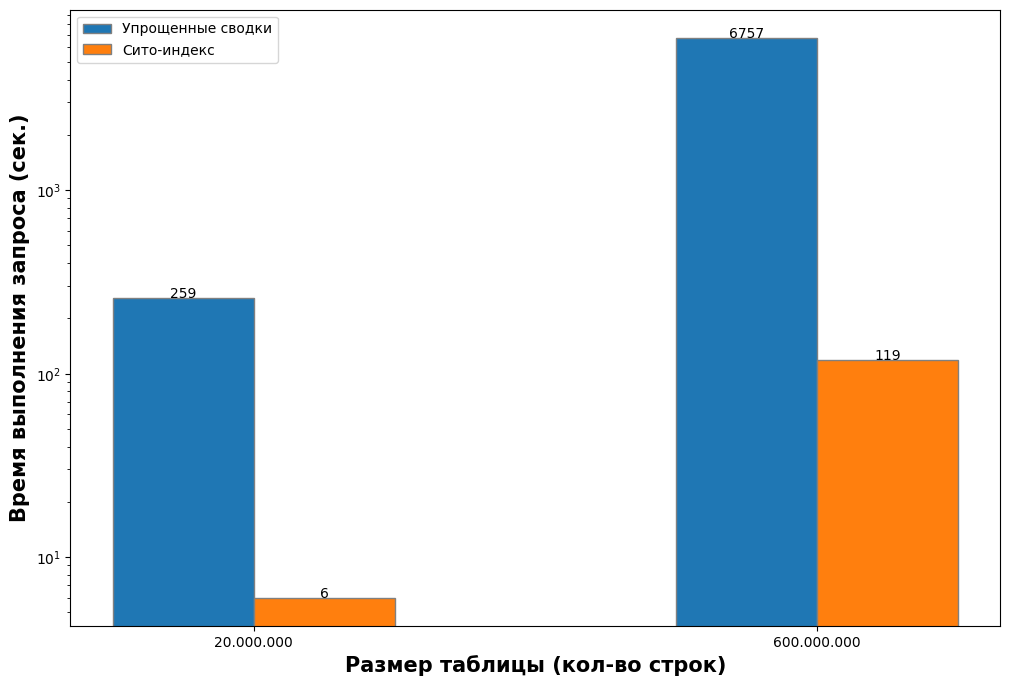
\includegraphics[scale=0.62]{2_range_query.png}
    \caption{\centering{Сравнение времени выполнения интервального запроса с использованием упрощенных сводок и Сито-индекса на двух таблицах разного размера}}
\end{figure}

Стоит отметить, что созданный случай является наилучшим для Сито-индекса, так как почти каждый файл с данными в обеих наборах содержал значения дат в диапазоне с 1 января 1992 года по 1 января 2008 года, в то время как в действительности почти каждый файл сдержал все даты с 1 января 1992 года по 1 января 1998 года и все даты с 1 января 2007 года по 1 января 2008 года. Интервальный запрос был выполнен с предикатом $1$ января $2003$г. $\leq shipdate \leq 31$ января $2003$г., а точечный с предикатом $shipdate = 1$ января $2003$г. Таким образом, упрощенные сводки допускали чтение всех файлов с данными, в то время как Сито-индекс пропускал чтение почти всех файлов.

В сценарии же, когда выполнение запроса с предикатом подразумевало чтение всех фалов с данными, время выполнения запроса было одинаковым для Сито-индекса и упрощенных сводок.

Далее представлено сравнение времени построения индекса для двух наборов данных.

\begin{figure}[h]
    \centering
    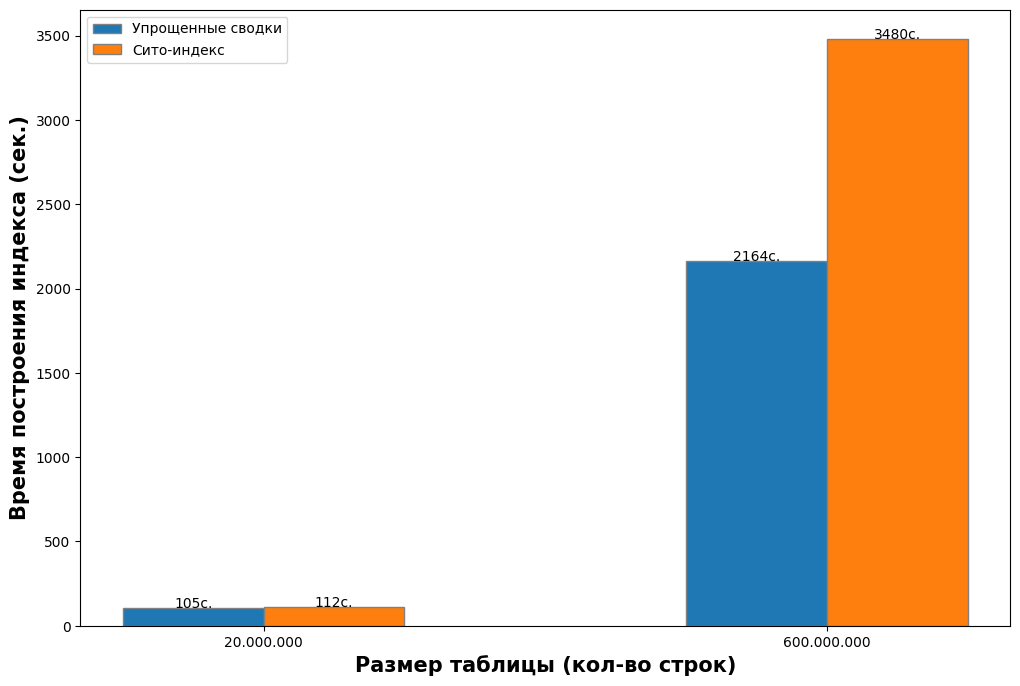
\includegraphics[scale=0.62]{3_build_time.png}
    \caption{\centering{Сравнение времени построения упрощенных сводок и Сито-индекса на двух таблицах разного размера}}
\end{figure}

Построение Сито-индекса занимает больше времени ввиду большей вычислительной сложности алгоритма построения индекса. Однако является сопоставимым с построением упрощенных сводок, так как для построения упрощенных сводок необходимо прочитать весь индексируемый атрибут, в то время как для построения Сито-индекса его необходимо еще и отсортировать.


\newpage
\section*{Выводы}
\addcontentsline{toc}{section}{Выводы}

Благодаря внедрению Сито-индекса в систему для доступа к данным с открытым исходным кодом Apache Hudi удалось добиться прироста скорости выполнения точечных запросов на порядки, а интервальных запросов на порядок для тех сценариев использования, когда имеющиеся в Apache Hudi фильтры для отсеивания нерелевантных файлов --- упрощенные сводки были не способны отсеивать файлы.

В худших же сценариях использования Сито-индекса время выполнения запросов с данной структурой было не больше времени выполнения тех же запросов, но с использованием упрощенных сводок.
